\begin{center}
\large Experimento: \textbf{Amplificador de instrumentação utilizando amplificadores operacionais}
\end{center}

\setlength{\abovedisplayskip}{-10pt}
\setlength{\belowdisplayskip}{-10pt}

\section{Introdução}


O presente relatório visa detalhar o experimento laboratorial realizado na disciplina laboratório de circuitos eletrônicos no dia 01 de outubro de 2019 sobre amplificador de instrumentação utilizando amplificadores operacionais (AMPOPs), mais especificamente os do circuito integrado LM741. Para isso, foi necessário o cálculo teórico dos ganhos diferenciais e de modo comum de ambas configurações, posteriormente durante a prática foi realizado medições para se verificar os ganhos obtidos.

A atividade foi dividida em duas parte, uma na análise com o amplificador de instrumentação com buffers, o que já garante o efeito desejado de um amplificador diferencial e a outra com um circuito com ganho melhorado utilizando a forma completa deste circuito, os esquemas dos circuitos (\ref{ckt:1} e \ref{ckt:2}) podem ser visualizados abaixo.


\begin{figure}[H]
\begin{center}
\begin{tikzpicture} [ american, ]
    \draw (0,0) node[op amp,yscale=-1] (opamp1) {}
    (opamp1.-) -- (-1.5,-0.5)
    (opamp1.+) -- (-1.5,0.5)  node[left] {$V_{2}$}
    (opamp1.out) --  (1.5,0) %node[right] {$V_o$}
    %(opamp1.up) --++(0,1.005) node[vcc]{15\,\textnormal{V}}
    %(opamp1.down) --++(0,-1.005) node[vee]{-15\,\textnormal{V}}
    (-1.5,-0.5) -- (-1.5,-1.5) -- (1.5,-1.5)
    (1.5,-1.5) to[short,-*] (1.5,0);
    
    
    \draw (0,-3.5) node[op amp] (opamp2) {}
    (opamp2.+) -- (-1.5,-4)  node[left] {$V_{1}$}
    (opamp2.-) -- (-1.5,-3)
    (opamp2.out) --  (1.5,-3.5) %node[right] {$V_o$}
    %(opamp2.up) --++(0,0.005) node[vcc]{15\,\textnormal{V}}
    %(opamp2.down) --++(0,-0.005) node[vee]{-15\,\textnormal{V}}
    (-1.5,-3) -- (-1.5,-2) -- (1.5,-2)
    (1.5,-2) to[short,-*] (1.5,-3.5)
    ;
    
    \draw (6,-1.75) node[op amp] (opamp3) {}
    (opamp3.+) -- (4,-2.25)
    (opamp3.-) -- (4,-1.25)
    (opamp3.out) --  (7.5,-1.75) node[right] {$V_o$}
    %(opamp2.up) --++(0,0.005) node[vcc]{15\,\textnormal{V}}
    %(opamp2.down) --++(0,-0.005) node[vee]{-15\,\textnormal{V}}
    ;

    \draw (1.5,0) to[R,l=$R_1$, -*] (4,0)
    (1.5,-3.5) to[R,l_=$R_{1}^{'}$, -*] (4,-3.5)
    (4,0) -- (4,-1.25)
    (4,-3.5) -- (4,-2.25)
    (4,0) to[R,l=$R_F$] (7,0)
    (4,-3.5) to[R,l_=$R_{F}^{'}$] (7,-3.5)
    (7,-3.5) node[ground]{}
    (7,0) to[short,-*] (7,-1.75)
    ;

\end{tikzpicture}

\end{center}
\caption{Amplificador de instrumentação com \textit{buffers} ($R_{1}=R_{1}^{'}=R_{F}=R_{F}^{'}= 12k \ohm$).}
\label{ckt:1} 
\end{figure}
\begin{figure}[H]
\begin{center}
\begin{tikzpicture} [ american, ]
    \draw (-3.5,-3.75) to[pR, l_=$50k \ohm$] (-3.5,-1.75)
    (-3.5,0.25) to[R,l=$1k \ohm$] (-3.5,-1.75)
    (-3.5,-3.75) to[short,-*] (-1.5,-3.75)
    (-3.5,0.25) to[short,-*] (-1.5,0.25)
    (-4,-2.75) -- (-4.25,-2.75) -- (-4.25,-1.75) -- (-3.5,-1.75)
    ;
    
    \draw (0,0.75) node[op amp,yscale=-1] (opamp1) {}
    (opamp1.-) -- (-1.5,0.25)
    (opamp1.+) -- (-1.5,1.25)  node[left] {$V_{2}$}
    (opamp1.out) --  (1.5,0.75) %node[right] {$V_o$}
    %(opamp1.up) --++(0,1.005) node[vcc]{15\,\textnormal{V}}
    %(opamp1.down) --++(0,-1.005) node[vee]{-15\,\textnormal{V}}
    (-1.5,0.25) -- (-1.5,-1.25) 
    (-1.5,-1.25) to[R,l=$27k \ohm$] (1.5,-1.25)
    (1.5,-1.25) to[short,-*] (1.5,0.75);
    
    
    \draw (0,-4.25) node[op amp] (opamp2) {}
    (opamp2.+) -- (-1.5,-4.75)  node[left] {$V_{1}$}
    (opamp2.-) -- (-1.5,-3.75)
    (opamp2.out) --  (1.5,-4.25) %node[right] {$V_o$}
    %(opamp2.up) --++(0,0.005) node[vcc]{15\,\textnormal{V}}
    %(opamp2.down) --++(0,-0.005) node[vee]{-15\,\textnormal{V}}
    (-1.5,-3.75) -- (-1.5,-2.25) 
    (-1.5,-2.25) to[R,l_=$27k \ohm$] (1.5,-2.25)
    (1.5,-2.25) to[short,-*] (1.5,-4.25)
    ;
    
    \draw (6,-1.75) node[op amp] (opamp3) {}
    (opamp3.+) -- (4,-2.25)
    (opamp3.-) -- (4,-1.25)
    (opamp3.out) --  (7.5,-1.75) node[right] {$V_o$}
    %(opamp2.up) --++(0,0.005) node[vcc]{15\,\textnormal{V}}
    %(opamp2.down) --++(0,-0.005) node[vee]{-15\,\textnormal{V}}
    ;

    \draw (1.5,0.75) to[R,l=$R_1$, -*] (4,0.75)
    (1.5,-4.25) to[R,l_=$R_{1}^{'}$, -*] (4,-4.25)
    (4,0.75) -- (4,-1.25)
    (4,-4.25) -- (4,-2.25)
    (4,0.75) to[R,l=$R_F$] (7,0.75)
    (4,-4.25) to[R,l_=$R_{F}^{'}$] (7,-4.25)
    (7,-4.25) node[ground]{}
    (7,0.75) to[short,-*] (7,-1.75)
    ;

\end{tikzpicture}

\end{center}
\caption{Amplificador de instrumentação completo ($R_{1}=R_{1}^{'}=R_{F}=R_{F}^{'}= 12k \ohm$).}
\label{ckt:2} 
\end{figure}

A prática tem o objetivo de comparar os valores de ganho diferencial ($A_d$) e de modo comum ($A_{CM}$) de ambos os circuitos e notar a relação existente de modo a observar que o ganho diferencial total do circuito \ref{ckt:2} é muito melhor que o ganho diferencial do circuito \ref{ckt:1}.

Primeiramente o circuito da figura \ref{ckt:1}, é baseado em buffers para que a tensão saída dependa apenas dos valores de tensão de entrada e que a resistência de entrada seja infinita. Assim nesta configuração obtêm-se um ganho diferencial unitário e um ganho de modo comum nulo. Devido não existir no mercado resistores perfeitamente iguais, vai existir um ganho de modo comum diferente de zero devido a esse motivo, esse ganho foi medido teoricamente e observado no multímetro digital de bancada. Já o circuito da figura \ref{ckt:1} foi adicionado amplificadores não-inversores ao invés de buffers, porém pela configuração mostrada, esses amplificadores não são mais tratados como amplificadores não-inversores, devido não possui uma referência terra entre os resistores da entrada inversora. Foi posto um potenciômetro para analisar o ganho diferencial mínimo e máximo do sistema, percebendo a diferença entre os valores de $A_d$ mostrados em ambas configurações analisadas. É notado que os ganhos de modo comum serão semelhantes na ordem de grandeza dos circuitos para ambos os circuitos.       

O osciloscópio digital foi utilizado para medir as formas de onda na entrada e na saída do amplificador de instrumentação, como forma de comparar os valores e comprovar os resultados teóricos.


\section{Análise Teórica}

Os circuitos projetados para a instrumentação são normalmente sensíveis, necessitando de uma característica diferencial para eliminar o ruído do sinal de entrada; alta impedância de entrada para que não se altere o fenômeno a ser medido; necessidade de um ganho grande; e devem ser lineares, permitindo ser aplicados com AMPOPs.

\begin{figure}[H]
\begin{center}
\begin{tikzpicture} [ american, ]
    \draw (6,-1.75) node[op amp] (opamp3) {}
    (opamp3.+) -- (4,-2.25)
    (opamp3.-) -- (4,-1.25)
    (opamp3.out) --  (7.5,-1.75) node[right] {$V_o$}
    %(opamp2.up) --++(0,0.005) node[vcc]{15\,\textnormal{V}}
    %(opamp2.down) --++(0,-0.005) node[vee]{-15\,\textnormal{V}}
    ;

    \draw (1.5,0) node[left] {$V_2$} to[R,l=$R_1$, o-*] (4,0)
    (1.5,-3.5) node[left] {$V_1$} to[R,l_=$R_{3}$, o-*] (4,-3.5)
    (4,0) -- (4,-1.25)
    (4,-3.5) -- (4,-2.25)
    (4,0) to[R,l=$R_2$] (7,0)
    (4,-3.5) to[R,l_=$R_{4}$] (7,-3.5)
    (7,-3.5) node[ground]{}
    (7,0) to[short,-*] (7,-1.75)
    ;

\end{tikzpicture}

\end{center}
\caption{Amplificador diferencial com AMPOPs.}
\label{ckt:3} 
\end{figure}

O uso de amplificador diferencial com AMPOP surge como uma primeira solução para o problema. Segundo o circuito da figura \ref{ckt:3}, devido a sua linearidade, o teorema da superposição pode ser utilizado para encontrar a saída do circuito por meio da contribuição individual de cada uma das entradas, implicando na expressão abaixo:

\begin{center}
\begin{equation} \label{dif:1}
        V_o = \frac{R_4}{R_3+R_4}\frac{R_1+R_2}{R_1}V_1 - \frac{R_2}{R_1}V_2
\end{equation}
\end{center}

Como amplificador diferencial, quererá determinar $A_d$ e $A_{CM}$ de forma que a saída fique na forma:

\begin{center}
\begin{equation} \label{dif:2}
        V_o = A_d(V_1-V_2)+A_{CM}\left(\frac{V_1+V_2}{2}\right)
\end{equation}
\end{center}

Comparando os elementos de \ref{dif:1} com \ref{dif:2}, obtém-se expressões para $A_d$ e $A_{CM}$:

\begin{center}
\begin{equation} \label{ad:1}
        A_d = \frac{1}{2}\left(\frac{R_4}{R_3+R_4}\frac{R_1+R_2}{R_1} + \frac{R_2}{R_1}\right)
\end{equation}
\end{center}

\begin{center}
\begin{equation} \label{acm:1}
        A_{CM} = \left(\frac{R_4}{R_3+R_4}\frac{R_1+R_2}{R_1} - \frac{R_2}{R_1}\right)
\end{equation}
\end{center}

Nas condições ideais de operação é desejado um ganho de modo comum nulo, que pode ser obtido com a seguinte relação:

\begin{center}
\begin{equation} \label{r:1}
        \frac{R_1}{R_2} = \frac{R_3}{R_4}
\end{equation}
\end{center}

Normalmente é escolhido $R_1=R_3$ e $R_2=R_4$, permitindo anular o ganho de modo comum e permitindo que o ganho diferencial seja:

\begin{center}
\begin{equation} \label{ad:2}
        A_d = \frac{R_2}{R_1}
\end{equation}
\end{center}

E a expressão final para o circuito:

\begin{center}
\begin{equation} \label{ad:2}
        V_o = \frac{R_2}{R_1}(V_1-V_2)
\end{equation}
\end{center}

Esse circuito possui uma resistência de saída nula, uma vez que a saída é ligada na saída do AMPOP. Porém a resistência de entrada diferencial será $2\times R_1$. Uma topologia utilizada para solucionar esse problema é utilizar dois \textit{buffers}, um para cada entrada, garantindo uma resistência de entrada infinita, assim como no circuito da figura \ref{ckt:1}.

Porém o custo do circuito é aumentado por conta dos novos AMPOPs. A alternativa é aproveitar os dois novos AMPOPs para realizar um primeiro estágio de amplificação simétrico em cada uma das entradas.

Assim, utiliza-se dois amplificadores não-inversores modificados (sem a conexão terra) de acordo com a topologia do circuito da figura \ref{ckt:4}.

\begin{figure}[H]
\begin{center}
\begin{tikzpicture} [ american, ]
    \draw (-3.5,-3.75) to[R, l_=$R_1$] (-3.5,-1.75)
    (-3.5,0.25) to[R,l=$R_1$] (-3.5,-1.75)
    (-3.5,-3.75) to[short,-*] (-1.5,-3.75)
    (-3.5,0.25) to[short,-*] (-1.5,0.25)
    ;
    
    \draw (0,0.75) node[op amp,yscale=-1] (opamp1) {}
    (opamp1.-) -- (-1.5,0.25)
    (opamp1.+) -- (-1.5,1.25)  node[left] {$V_{2}$}
    (opamp1.out) --  (1.5,0.75) %node[right] {$V_o$}
    %(opamp1.up) --++(0,1.005) node[vcc]{15\,\textnormal{V}}
    %(opamp1.down) --++(0,-1.005) node[vee]{-15\,\textnormal{V}}
    (-1.5,0.25) -- (-1.5,-1.25) 
    (-1.5,-1.25) to[R,l=$R_2$] (1.5,-1.25)
    (1.5,-1.25) to[short,-*] (1.5,0.75);
    
    
    \draw (0,-4.25) node[op amp] (opamp2) {}
    (opamp2.+) -- (-1.5,-4.75)  node[left] {$V_{1}$}
    (opamp2.-) -- (-1.5,-3.75)
    (opamp2.out) --  (1.5,-4.25) %node[right] {$V_o$}
    %(opamp2.up) --++(0,0.005) node[vcc]{15\,\textnormal{V}}
    %(opamp2.down) --++(0,-0.005) node[vee]{-15\,\textnormal{V}}
    (-1.5,-3.75) -- (-1.5,-2.25) 
    (-1.5,-2.25) to[R,l_=$R_2$] (1.5,-2.25)
    (1.5,-2.25) to[short,-*] (1.5,-4.25)
    ;
    
    \draw (6,-1.75) node[op amp] (opamp3) {}
    (opamp3.+) -- (4,-2.25)
    (opamp3.-) -- (4,-1.25)
    (opamp3.out) --  (7.5,-1.75) node[right] {$V_o$}
    %(opamp2.up) --++(0,0.005) node[vcc]{15\,\textnormal{V}}
    %(opamp2.down) --++(0,-0.005) node[vee]{-15\,\textnormal{V}}
    ;

    \draw (1.5,0.75) to[R,l=$R_3$, -*] (4,0.75)
    (1.5,-4.25) to[R,l_=$R_3$, -*] (4,-4.25)
    (4,0.75) -- (4,-1.25)
    (4,-4.25) -- (4,-2.25)
    (4,0.75) to[R,l=$R_4$] (7,0.75)
    (4,-4.25) to[R,l_=$R_4$] (7,-4.25)
    (7,-4.25) node[ground]{}
    (7,0.75) to[short,-*] (7,-1.75)
    ;

\end{tikzpicture}

\end{center}
\caption{Amplificador de instrumentação completo.}
\label{ckt:4} 
\end{figure}

Considerando um ganho de modo comum não nulo e de valor realizável pela equação \ref{acm:1}, a expressão final para a saída baseada no circuito da figura \ref{ckt:4} será (a mesma expressão pode ser adaptada para o circuito da figura \ref{ckt:2} utilizado na prática):

\begin{center}
\begin{equation} \label{vo:1}
        V_o = \frac{R_4}{R_3}\left( 1+\frac{R_2}{R_1}\right)(V_1-V_2)+A_{CM}\left(\frac{V_1+V_2}{2}\right)
\end{equation}
\end{center}

Assim, permitindo que o ganho diferencial seja amplificado e que o ganho de modo comum permaneça constante.

\subsection{Resultados Teóricos}

Devido a faixa de tolerância dos resistores, a diretiva da equação \ref{r:1} não poderá ser obedecida fielmente, gerando divergência nos valores das resistências e implicando em um ganho de modo comum devido a assimetria.

Dessa forma, para que a teoria corrobore com a prática, se faz necessário utilizar os valores reais medidos de resistência de cada resistor. Os valores de resistência dos resistores podem ser conferidos na tabela \ref{tab:1} e a resistência do potenciômetro varia entre $R_{p,min} = 2.64 \ohm$ e $R_{p,max} = 56.91k \ohm$. 

\subsubsection{Amplificador de instrumentação com \textit{buffers}}

Para o circuito da figura \ref{ckt:1} foram testados o ganho diferencial e de modo comum. Eles podem ser encontrados, respectivamente, utilizando as equações \ref{ad:1} e \ref{acm:1}. Dessa forma, tem-se:


\begin{equation} \label{adacm:1}
\begin{aligned}
        A_d = 0.99536 V/V \\ 
        A_{CM} = 0.0024176 V/V
\end{aligned}
\end{equation}

Portanto, no que confere o ganho de modo comum, sendo as entradas $V_1=V_2=0.5 \times 20 \times sen(2 \pi \times 100t) V$, pela fórmula \ref{dif:2} espera-se uma saída de $V_o = 0.5 \times 48.352 \times sen(2 \pi \times 100t) mV$

Já para o ganho diferencial, sendo as entradas $V_2=0$ e $V_1=0.5 \times 9.68 \times sen(2 \pi \times 100t) V$, pela fórmula \ref{dif:2} espera-se uma saída de $V_o = 0.5 \times 9.635 \times sen(2 \pi \times 100t) V$

\subsubsection{Amplificador de instrumentação completo}

Para o circuito da figura \ref{ckt:2} foram testados o ganho diferencial e de modo comum para as duas condições limites do potenciômetro. Eles podem ser encontrados, respectivamente, utilizando as equações \ref{ad:3} e \ref{acm:1}. Dessa forma, tem-se:

\begin{center}
\begin{equation} \label{ad:3}
        A_d = \frac{R_4}{R_3}\left( 1+\frac{R_2}{R_1}\right)
\end{equation}
\end{center}

Observa-se na equação \ref{vo:1} que o ganho de modo comum não se altera com base no valor que foi previsto anteriormente na equação \ref{adacm:1}. 

Considerando o valor mínimo de resistência do potenciômetro, obtém-se o valor máximo do ganho diferencial ($A_{d,max}$). Já para o valor máximo da resistência do potenciômetro, obtém-se o valor mínimo do ganho diferencial ($A_{d,min}$). Seus valores serão:

\begin{equation} \label{adacm:2}
\begin{aligned}
        A_{d,min} = 1.9182 V/V \\ 
        A_{d,max} = 54.9602 V/V
\end{aligned}
\end{equation}

Por fim, para o ganho diferencial máximo, sendo as entradas $V_2=0$ e $V_1=0.5 \times 200 \times sen(2 \pi \times 100t) mV$ e com a resistência mínima do potenciômetro, pela fórmula \ref{dif:2} espera-se uma saída de $V_o = 0.5 \times 10.99 \times sen(2 \pi \times 100t) V$

E para o ganho diferencial mínimo, sendo as entradas $V_2=0$ e $V_1=0.5 \times 10 \times sen(2 \pi \times 100t) V$ e com a resistência mínima do potenciômetro, pela fórmula \ref{dif:2} espera-se uma saída de $V_o = 0.5 \times 19.182 \times sen(2 \pi \times 100t) V$

\section{Resultados e discussão}

Para encontrar todos os resultados necessários para comprovar a teoria, a prática foi dividida em algumas etapas, sendo elas:

\begin{itemize}
    \item Medição de todos resistores utilizados;
    \item Montar o circuito da figura \ref{ckt:1} e aplicar $V_1 = V_2 = 10 \times sen (2\pi100t)$ V, medir o $A_{CM}$ com multímetro de bancada;
    \item Aplicar agora $V_2 = 0$ $V_1 = 5 \times sen (2\pi100t)$ V, medir o $A_{d}$ com osciloscópio;
    \item Montar o circuito da figura \ref{ckt:2} e repetir os passos anteriores, aplicando os valores mínimo e máximo do potenciômetro;
\end{itemize}

De inicio foi utilizado o multímetro digital de bancada para medir os resistores disponíveis, tais valores são dispostos na tabela a seguir:


\begin{table}[H]
\centering
\begin{tabular}{|c|c|c|c|c|c|c|c}
\hline
\textbf{$R_1$} & \textbf{$R_{1}^{'}$} & \textbf{$R_F$} & \textbf{$R_{F}^{'}$} & \textbf{$R_{27k,v1}$} & \textbf{$R_{27k,v2}$} & \textbf{$R_{1k}$} \\ \hline
11,805 k\ohm & 11,854 k\ohm & 11,736 k\ohm & 11,842 k\ohm & 27,196 k\ohm & 26,620 k\ohm & 0,9887 k\ohm \\ \hline
\end{tabular}
\caption{Valores de resistências medidas para os resistores utilizados na prática.}
\label{tab:1}
\end{table}

Com $R_{27k,v1}$ e $R_{27k,v2}$, respectivamente o valor dos resistores de $27k \ohm$ associados às entradas $V_1$ e $V_2$ e $R_{1k}$ o resistor de $1k \ohm$.

Para a medição do ganho de modo comum ($A_{CM}$) da figura \ref{ckt:1}, primeiramente as tensões de entrada foram colocadas no mesmo potencial de $20V_{PP}$ e $100Hz$, com auxílio do multímetro de bancada foi medido o potencial de saída do circuito ($V_o$) de modo que obteve-se um valor de $V_o = 0,04681 V_{PP}$, com isso foi obtido o valor de $A_{CM}$. Os resultados dos valores teóricos e medidos de $A_{CM}$ são mostrados na tabela a seguir.


\begin{table}[H]
\centering
\begin{tabular}{c|c|c|c|}
\cline{2-4}
\textbf{} & \textbf{Valor Ideal} & \textbf{Valor Teórico} & \textbf{Valor Medido} \\ \hline
\multicolumn{1}{|c|}{\textbf{$V_1 = V_2  =  20 V_{PP}$}} & 0 V/V & 0,0024176 V/V & 0,0023402 V/V \\ \hline
\end{tabular}
\caption{Valores teóricos e medidos de $A_{CM}$ para a figura \ref{ckt:1}}
\label{tab:2}
\end{table}


Para análise do ganho diferencial ($A_d$) do circuito da figura \ref{ckt:1} devemos colocar o potencial da primeira entrada ($V_1$) em $10V_{PP}$, já a tensão da segunda entrada deve ser aterrada, ou seja, $V_2 = 0V$, desta forma com ajuda do osciloscópio obteremos o valor da tensão de saída ($V_o$) como mostra a figura \ref{p2-out}.

\begin{figure}[H] 
\centering
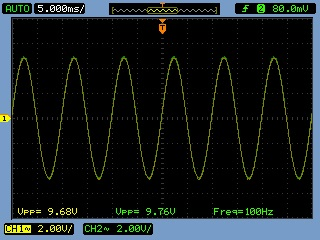
\includegraphics[scale=0.7]{imagens/AD1_CH12.jpg} 
\caption{Saída e entrada do amplificador de instrumentação, com $V_2=0$ e $V_1=5 sen(2\pi100t)V$}
\label{p2-out} 
\end{figure}

Com esses valores obtemos $A_d$, pelo o quociente da tensão de saída e entrada, como pode-se observar pela figura \ref{p2-out}, o valor de entrada é aproximadamente $V_1 = 9.68 V_{PP}$ os valores encontrados são mostrados na tabela de resultados a seguir.


\begin{table}[H]
\centering
\begin{tabular}{c|c|c|c|}
\cline{2-4}
\textbf{} & \textbf{Valor Ideal} & \textbf{Valor Teórico} & \textbf{Valor Medido} \\ \hline
\multicolumn{1}{|c|}{\textbf{$V_1 = 10 V_{PP}$ e $V_2 = 0V$ }} & 1 V/V & 0,9954 V/V & 0,9918V/V \\ \hline
\end{tabular}
\caption{Valores teóricos e medidos de $A_{d}$ para a figura \ref{ckt:1}.}
\label{tab:3}
\end{table}

Já para análise do amplificador instrumentação sem os buffers (figura \ref{ckt:2}), devemos medir a resistência mínima e máxima do potenciômetro que são respectivamente $R_{Pmin}=2,64\ohm$ e $R_{Pmáx}=56,91k\ohm$. Com esse valores obtemos o valores teóricos máximos e mínimos do ganho em modo comum para esse circuito. O processo de medição é basicamente o mesmo do circuito anterior, foi colocado $20V_{PP}$ no potencial das entradas ($V_1$ e $V_2$), de modo que no multímetro de banca foi medido o valor da tensão de saída, que foi de aproximadamente $V_{Omin} = V_{Omax} =17,87mV$.

Os valores do ganho em modo comum do circuito da figura \ref{ckt:2} são mostradas na tabela a baixo.

\begin{table}[H]
\centering
\begin{tabular}{c|c|c|c|}
\cline{2-4}
\textbf{} & \textbf{Valor Ideal} & \textbf{Valor Teórico} & \textbf{Valor Medido} \\ \hline
\multicolumn{1}{|c|}{\textbf{$V_1 = V_2  =  20 V_{PP}$}} & 0 V/V & 0,0024176 V/V & 0,0025272 V/V \\ \hline
\end{tabular}
\caption{Valores teóricos e medidos de $A_{CM}$ para a figura \ref{ckt:2}.}
\label{tab:4}
\end{table}

Percebe-se que os valores $A_{CM}$ são iguais ao amplificador de instrumentação com buffers, isso se deve que tanto o circuito da figura \ref{ckt:1}, quanto o circuito da figura \ref{ckt:2} proporciona resistência de entrada infinita, ou seja, em aberto. Com isso o ganho de em modo comum é aproximadamente nulo nos dois casos.  

Para medição de $A_{d,max}$, foi utilizado o mesmo procedimento que o circuito anterior, ou seja, devemos aterrar a segunda entrada de modo que ($V_2=0$), e aplicar um potencial tensão baixo ($V_1= 208mV_{PP}$) na entrada 1, devido o ganho ser diferente de 1 como no caso da figura \ref{ckt:1}. Dessa modo, foi possível obter o valor de tensão na saída e em seguida ($A_{d,max}$). A seguir a figura correspondente as medições realizadas no osciloscópio.

\begin{figure}[H] 
\centering
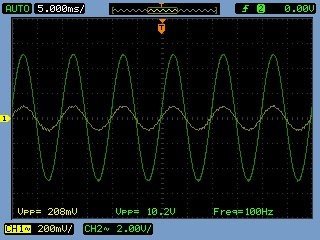
\includegraphics[scale=0.7]{imagens/AD2MAX_COM_FILTRO.jpg} 
\caption{Saída e entrada do amplificador de instrumentação, com $V_2=0$ e $V_1=200\times10^{-3} sen(2\pi100t)V$}
\label{p3-out} 
\end{figure}

Da mesma forma foi medido $A_{d,min}$, porém ao invés de $V_1= 208mV_{PP}$, será usado a tensão recomendada na aula, ou seja, $V_1= 10V_{PP}$, desse forma, a tensão de saída correspondente poderá ser vista na figura a seguir.

\begin{figure}[H] 
\centering
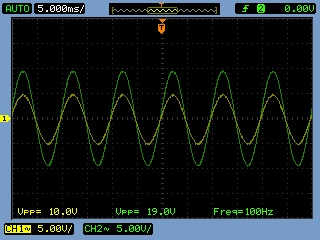
\includegraphics[scale=0.7]{imagens/AD2MIN.jpg} 
\caption{Saída e entrada do amplificador de instrumentação, com $V_2=0$ e $V_1=5sen(2\pi100t)V$}
\label{p3-out} 
\end{figure}


Desse modo, poderemos ver os valores de $A_{d,min}$ com $A_{d,max}$ medidos pela a tabela \ref{tab:5} seguinte.

\begin{table}[H]
\centering
\begin{tabular}{c|c|c|}
\cline{2-3}
\textbf{} & \textbf{Valor Teórico} & \textbf{Valor Medido} \\ \hline
\multicolumn{1}{|c|}{\textbf{$A_{d,min}$}} & 1,918 V/V & 1,92 V/V \\ \hline
\multicolumn{1}{|c|}{\textbf{$A_{d, max}$}} & 54,96 V/V & 51 V/V \\ \hline
\end{tabular}
\caption{Valores teóricos e medidos de $A_{d,min}$ e $A_{d,max}$  para a figura \ref{ckt:2}.}
\label{tab:5}
\end{table}

Podemos notar que o valor de $A_{d,max}$ medido divergiu um pouco do teórico, mas estar na mesma ordem de grandeza, isso foi devido ao fato que para pequenos valores de tensão na entrada, o ganho é perdido com os elementos internos do circuito. Também tinha-se muito ruído no sistema, foi preciso passar um filtro para estabilizar o sinal de entrada, como podemos notar na figura abaixo sem o filtro.

\begin{figure}[H] 
\centering
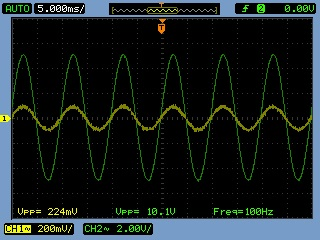
\includegraphics[scale=0.7]{imagens/AD2MAX_SEM_FILTRO.jpg} 
\caption{Saída e entrada do amplificador de instrumentação, com $V_2=0$ e $V_1=200\times10^{-3} sen(2\pi100t)V$}
\label{p4-out} 
\end{figure}

\section{Conclusões}

No primeiro circuito da prática, por mais que os \textit{buffers} de tensão resolvessem o problema da resistência de entrada não infinita, eles permitiam que as despesas financeiras com o circuito fossem maiores, pois se utiliza-se de três AMPOPs ao invés de um. 

Então os \textit{buffers} de tensão foram modificados para funcionarem como amplificadores não-inversores modificados no segundo circuito de forma a aumentar o ganho diferencial, porém sem o aumento do ganho de modo comum devido à remoção do terra de ambos os resistores de realimentação.

Dessa forma os resultados foram satisfatórios, permitindo comprovar a teoria em cada etapa da prática em laboratório.


\newpage

\section{Anexos}

\begin{figure}[H] 
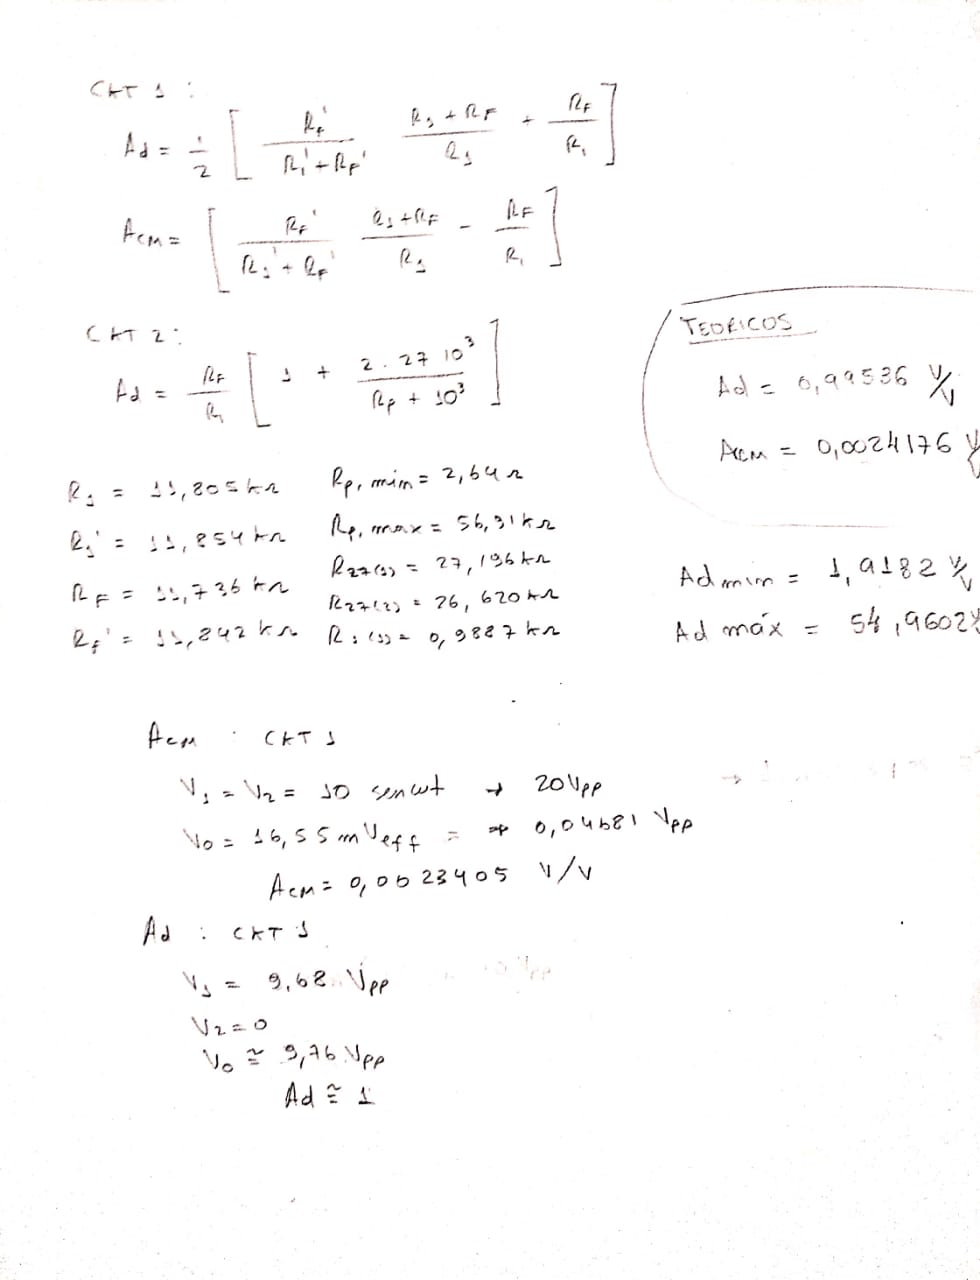
\includegraphics[scale=0.4]{imagens/calc1.jpeg} 
\centering
\caption{Folha 1 de cálculos da prática.}
\label{p5-2} 
\end{figure} 

\begin{figure}[H] 
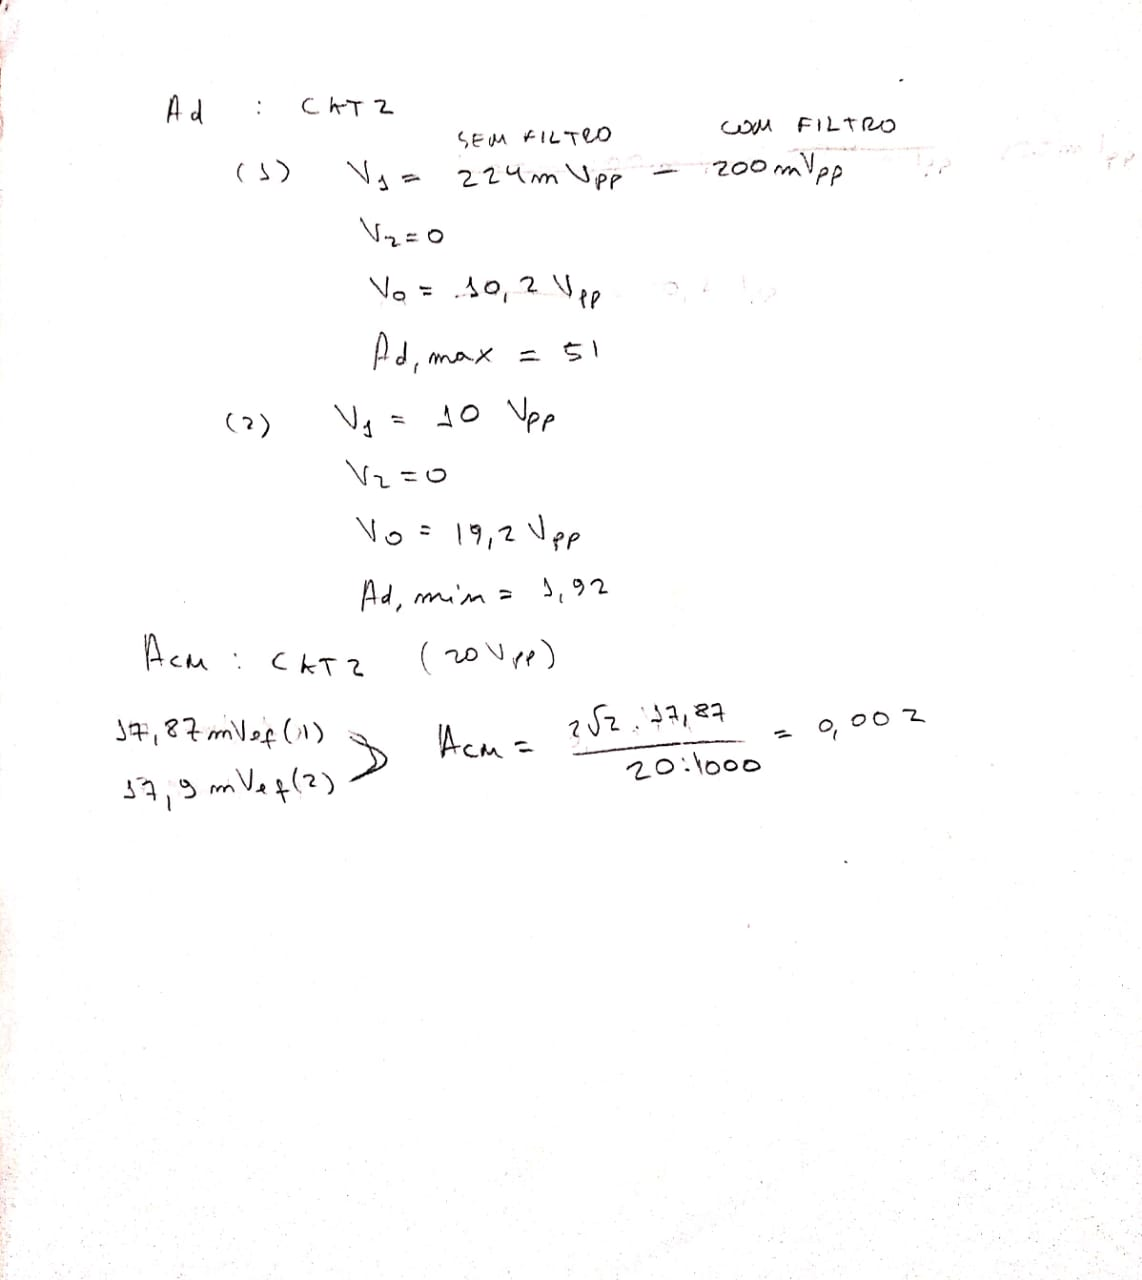
\includegraphics[scale=0.4]{imagens/calc2.jpeg} 
\centering
\caption{Folha 2 de cálculos da prática.}
\label{p5-2} 
\end{figure} 




     






